\documentclass{beamer}
\usepackage[utf8]{inputenc}
\usepackage{amsmath}
\usepackage{graphicx}
\usepackage{amsthm}
\graphicspath{ {./} } 

\title{Combination}
\author{Saleh ZareZade}
\date{2020}

\begin{document}

\frame{\titlepage}

\begin{frame} 
\frametitle{Contents} 
\tableofcontents
\end{frame} 

\section{1 Number of k-combinations}

\begin{frame}
\frametitle{Number of k-combinations}
The number of k-combinations from a given set S of n elements is often denoted in elementary combinatorics texts by C(n,k), or by a variation such as $C_{k}^{n}$,$ {}_{n}C_{k}$,${}^{n}C_{k}$, $C_{{n,k}}$ or even$ C_{n}^{k} $(the latter form was standard in French, Romanian, Russian, Chinese and Polish texts[citation needed]). The same number however occurs in many other mathematical contexts, where it is denoted by ${\tbinom {n}{k}}$ (often read as "n choose k"); notably it occurs as a coefficient in the binomial formula, hence its name binomial coefficient. One can define ${\tbinom {n}{k}} $for all natural numbers k at once by the relation:
$$(1+X)^n=\sum_{k\ge 0}{{\binom {n}{k}}X^k}$$
from which it is clear that
$${\binom {n}{0}}={\binom {n}{n}}=1$$
\end{frame}

\begin{frame}
\frametitle{Number of k-combinations}
To see that these coefficients count k-combinations from S, one can first consider a collection of n distinct variables$ X_s$ labeled by the elements s of S, and expand the product over all elements of S:
$$\prod_{s\in S}{(1+X_s);}$$
it has$ 2^n$ distinct terms corresponding to all the subsets of S, each subset giving the product of the corresponding variables$ X_s$. Now setting all of the$ X_s$ equal to the unlabeled variable X, so that the product becomes $(1 + X)^n$, the term for each k-combination from S becomes $X^k$, so that the coefficient of that power in the result equals the number of such k-combinations.\\
Binomial coefficients can be computed explicitly in various ways. To get all of them for the expansions up to $(1 + X)^n$, one can use (in addition to the basic cases already given) the recursion relation
$${\binom {n}{k}}={\binom {n-1}{k-1}}+{\binom {n-1}{k}}$$
\end{frame}

\begin{frame}
\frametitle{Number of k-combinations}
for $0 < k < n$, which follows from $ (1 + X)^n = (1 + X)^{n-1}(1+X)$; this leads to the construction of Pascal's triangle.
For determining an individual binomial coefficient, it is more practical to use the formula
$${\binom {n}{k}}=\frac{n(n-1)(n-2)\cdots (n-k)}{k!}$$
The numerator gives the number of k-permutations of n, i.e., of sequences of k distinct elements of S, while the denominator gives the number of such k-permutations that give the same k-combination when the order is ignored.\\
When k exceeds n/2, the above formula contains factors common to the numerator and the denominator, and canceling them out gives the relation
$${\binom {n}{k}}={\binom {n}{n-k}}$$
\end{frame}

\begin{frame}
\frametitle{Number of k-combinations}
for $0\le k\le n$. This expresses a symmetry that is evident from the binomial formula, and can also be understood in terms of k-combinations by taking the complement of such a combination, which is an $(n-k)$-combination.
Finally there is a formula which exhibits this symmetry directly, and has the merit of being easy to remember:
$${\binom {n}{k}}=\frac{n!}{(n-k)!k!}$$
where n! denotes the factorial of n. It is obtained from the previous formula by multiplying denominator and numerator by (n - k)!, so it is certainly inferior as a method of computation to that formula.\\
\end{frame}

\begin{frame}
\frametitle{Number of k-combinations}
The last formula can be understood directly, by considering the n! permutations of all the elements of S. Each such permutation gives a k-combination by selecting its first k elements. There are many duplicate selections: any combined permutation of the first k elements among each other, and of the final (n - k) elements among each other produces the same combination; this explains the division in the formula.\\
From the above formulas follow relations between adjacent numbers in Pascal's triangle in all three directions:
$${\binom {n}{k}}=
\begin{cases}
{\binom {n}{k-1}}\frac {n-k+1}{k} &\text{if } k>0\\
{\binom {n-1}{k}}\frac{n}{n-k}&\text{if }k<n\\
{\binom {n-1}{k-1}}\frac{n}{k}&\text{if } n,k>0
\end{cases}
$$
\end{frame}

\begin{frame}
\frametitle{Number of k-combinations}
Together with the basic cases ${\tbinom {n}{0}}=1={\tbinom {n}{n}}$, these allow successive computation of respectively all numbers of combinations from the same set (a row in Pascal's triangle), of k-combinations of sets of growing sizes, and of combinations with a complement of fixed size n - k.\\
\begin{figure}[h]
\caption{3-element subsets of a 5-element set}
\centering
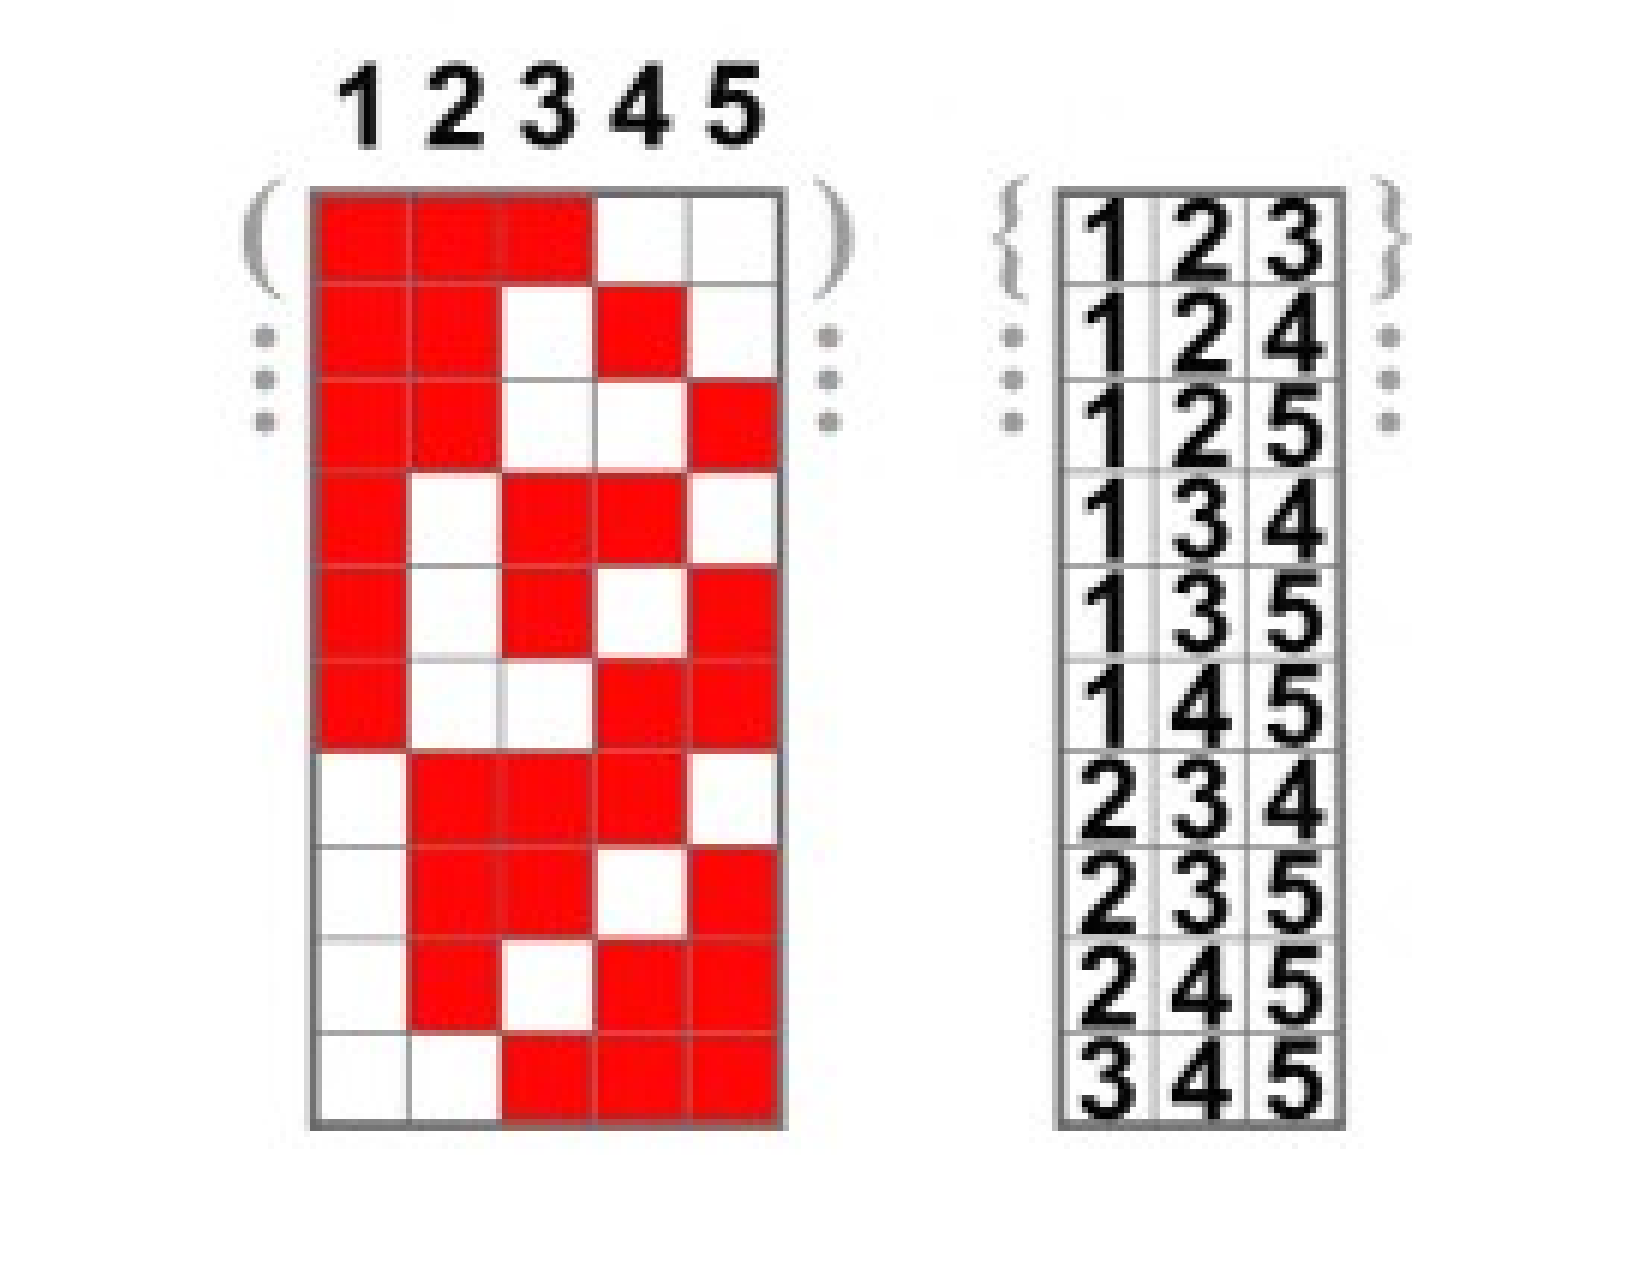
\includegraphics[width=0.5\textwidth]{1.pdf}
\end{figure}
\end{frame}

\subsection{1.1 Example of counting combinations}
\begin{frame}
\frametitle{Example of counting combinations}
As a specific example, one can compute the number of five-card hands possible from a standard fifty-two card deck as:
$${\binom {52}{5}}=\frac {52\times 51 \times 50 \times 49 \times 48}{5 \times 4 \times 3 \times 2 \times 1}=2,598,960$$\\
\end{frame}

\subsection{1.2 Enumerating k-combinations}
\begin{frame}
\frametitle{Enumerating k-combinations}
One can enumerate all k-combinations of a given set S of n elements in some fixed order, which establishes a bijection from an interval of ${\tbinom{n}{k}}$ integers with the set of those k-combinations. Assuming S is itself ordered, for instance $S = \{ 1, 2, \cdots, n \}$, there are two natural possibilities for ordering its k-combinations: by comparing their smallest elements first (as in the illustrations above) or by comparing their largest elements first. The latter option has the advantage that adding a new largest element to S will not change the initial part of the enumeration, but just add the new k-combinations of the larger set after the previous ones. Repeating this process, the enumeration can be extended indefinitely with k-combinations of ever larger sets. If moreover the intervals of the integers are taken to start at 0, then the k-combination at a given place i in the enumeration can be computed easily from i, and the bijection so obtained is known as the combinatorial number system. It is also known as "rank"/"ranking" and "unranking" in computational mathematics.\\
\end{frame}

\begin{frame}
\frametitle{Enumerating k-combinations}
There are many ways to enumerate k combinations. One way is to visit all the binary numbers less than $2^n$. Choose those numbers having k nonzero bits, although this is very inefficient even for small n (e.g. $ n = 20$ would require visiting about one million numbers while the maximum number of allowed k combinations is about 186 thousand for k = 10). The positions of these 1 bits in such a number is a specific k-combination of the set $\{ 1, …, n \}$. Another simple, faster way is to track k index numbers of the elements selected, starting with $\{ 0,\cdots, k-1\}$ (zero-based) or $\{1,\cdots ,k\}$ (one-based) as the first allowed k-combination and then repeatedly moving to the next allowed k-combination by incrementing the last index number if it is lower than $n-1$ (zero-based) or n (one-based) or the last index number x that is less than the index number following it minus one if such an index exists and resetting the index numbers after x to $\{x+1, x+2, …\}$.
\end{frame}

\section{2 Number of combinations with repetition}
\subsection{2.1 Example of counting multisubsets}
\begin{frame}
\frametitle{Example of counting multisubsets}
\footnotesize
{
\begin{table}[h]
\centering
\begin{tabular}{|c|c|c|c|}
\hline
No. & 3-Multiset & Eq. Solution & Stars and Bars \\
\hline
1&{1,1,1} &[3,0,0,0]&$\star \star \star |||$\\
\hline
2 &{1,1,2} &[2,1,0,0] &$\star \star |\star ||$\\
\hline
3&	{1,1,3}&	[2,0,1,0]&	$\star \star ||\star |$\\
\hline
4&	{1,1,4}&	[2,0,0,1]&	$\star \star |||\star$ \\
\hline
5&	{1,2,2}&	[1,2,0,0]&	$\star |\star \star ||$\\
\hline
6&	{1,2,3}&	[1,1,1,0]&	$\star |\star |\star |$\\
\hline
7&	{1,2,4}&	[1,1,0,1]&	$\star |\star ||\star$ \\
\hline
8&	{1,3,3}&	[1,0,2,0]&	$\star ||\star \star |$\\
\hline
9&	{1,3,4}&	[1,0,1,1]& $\star ||\star |\star$ \\
\hline
10&	{1,4,4}&	[1,0,0,2]&	$\star |||\star \star$ \\
\hline
11&	{2,2,2}&	[0,3,0,0]&	$|\star \star \star ||$\\
\hline
12&	{2,2,3}&	[0,2,1,0]&	$|\star \star |\star |$\\
\hline
13&	{2,2,4}&	[0,2,0,1]&	$|\star \star ||\star$ \\
\hline
14&	{2,3,3}&	[0,1,2,0]&	$|\star |\star \star |$\\
\hline
15&	{2,3,4}&	[0,1,1,1]&	$|\star |\star |\star$ \\
\hline
16&	{2,4,4}&	[0,1,0,2]&	$|\star ||\star \star$ \\
\hline
17&	{3,3,3}&	[0,0,3,0]&	$||\star \star \star |$\\
\hline
18&	{3,3,4}&	[0,0,2,1]&	$||\star \star |\star$ \\
\hline
19&	{3,4,4} &	[0,0,1,2]&	$||\star |\star \star$ \\
\hline 
20 &	{4,4,4} &	[0,0,0,3] &$|||\star \star \star$ \\
\hline
\end{tabular}
\end{table}
}
\end{frame}

\section{References}
\begin{frame}{Bibliography}
\frametitle{References}
\begin{itemize}
\item[1]
Benjamin, Arthur T.; Quinn, Jennifer J. (2003), Proofs that Really Count: The Art of Combinatorial Proof, The Dolciani Mathematical Expositions 27, The Mathematical Association of America, ISBN 978-0-88385-333-7
\item[2]
Brualdi, Richard A. (2010), Introductory Combinatorics (5th ed.), Pearson Prentice Hall, ISBN 978-0-13-602040-0
\item[3]
Erwin Kreyszig, Advanced Engineering Mathematics, John Wiley\& Sons, INC, 1999.
\item[4]
Mazur, David R. (2010), Combinatorics: A Guided Tour, Mathematical Association of America, ISBN 978-0-88385-762-5
\item[5]
Ryser, Herbert John (1963), Combinatorial Mathematics, The Carus Mathematical Monographs 14, Mathematical Association of America
\item[6]
https://en.wikipedia.org/wiki/Combination$\sharp$Number\_of\_k-combinations
\end{itemize}
\end{frame}

\end{document}